\documentclass{article}
\usepackage[hmargin=0.5in, vmargin=0.5in]{geometry}
\usepackage[hidelinks]{hyperref}
\usepackage{pdfpages}

\title{CS216 Final Project - Poker Recognize}
\author{Luis Hsu, Jeng-Hsun Ho}
\date{Luis' version}

\begin{document}
\maketitle

\setlength{\fboxrule}{0pt}

\section*{Overview}

In this project, we're going to recognize poker cards from an image. Before testing, we'll prepare several images of poker cards as templates, and being used to train the matcher. Then, we'll take an image to test, and output the recognization result of matched card. The project seems like a simple application, however, it needs to combine several techniques we learned from this course. Combining these skills is the main value that make this project suitable as the final evaluation after taking this course.

\section*{Data Sets}

For templates, we use several poker cards from a standard Bicycle Playing Cards, which are the spades from 2 to 10, club 2, diamond K, heart 5, and heart J.\\
The set of spades is used to check if the application can distinguish the cards of different numbers from the same shape.\\
The cards of diamond, club and hearts are used for recognize different shapes.\\
\includegraphics[scale=0.08]{IMG_1493.JPG}
\\
To get the template image, we use a scanner to scan cards for high resolution images. Here comes some examples below.\\
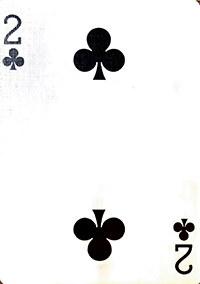
\includegraphics[scale=0.5]{club2.png}
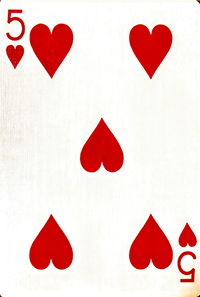
\includegraphics[scale=0.5]{heart5.png}
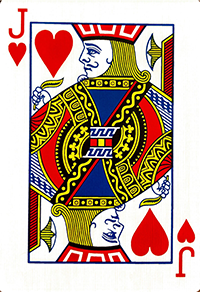
\includegraphics[scale=0.5]{heartJ.png}
\\\\
The test images are taken with a webcam that set on a certain distance above a plain table, and the test items are putting on it, as the picture shown.\\
\includegraphics[scale=0.08, angle=-90]{IMG_1496.JPG}
\\
Then we use VLC Player to capture the test image from the webcam.\\
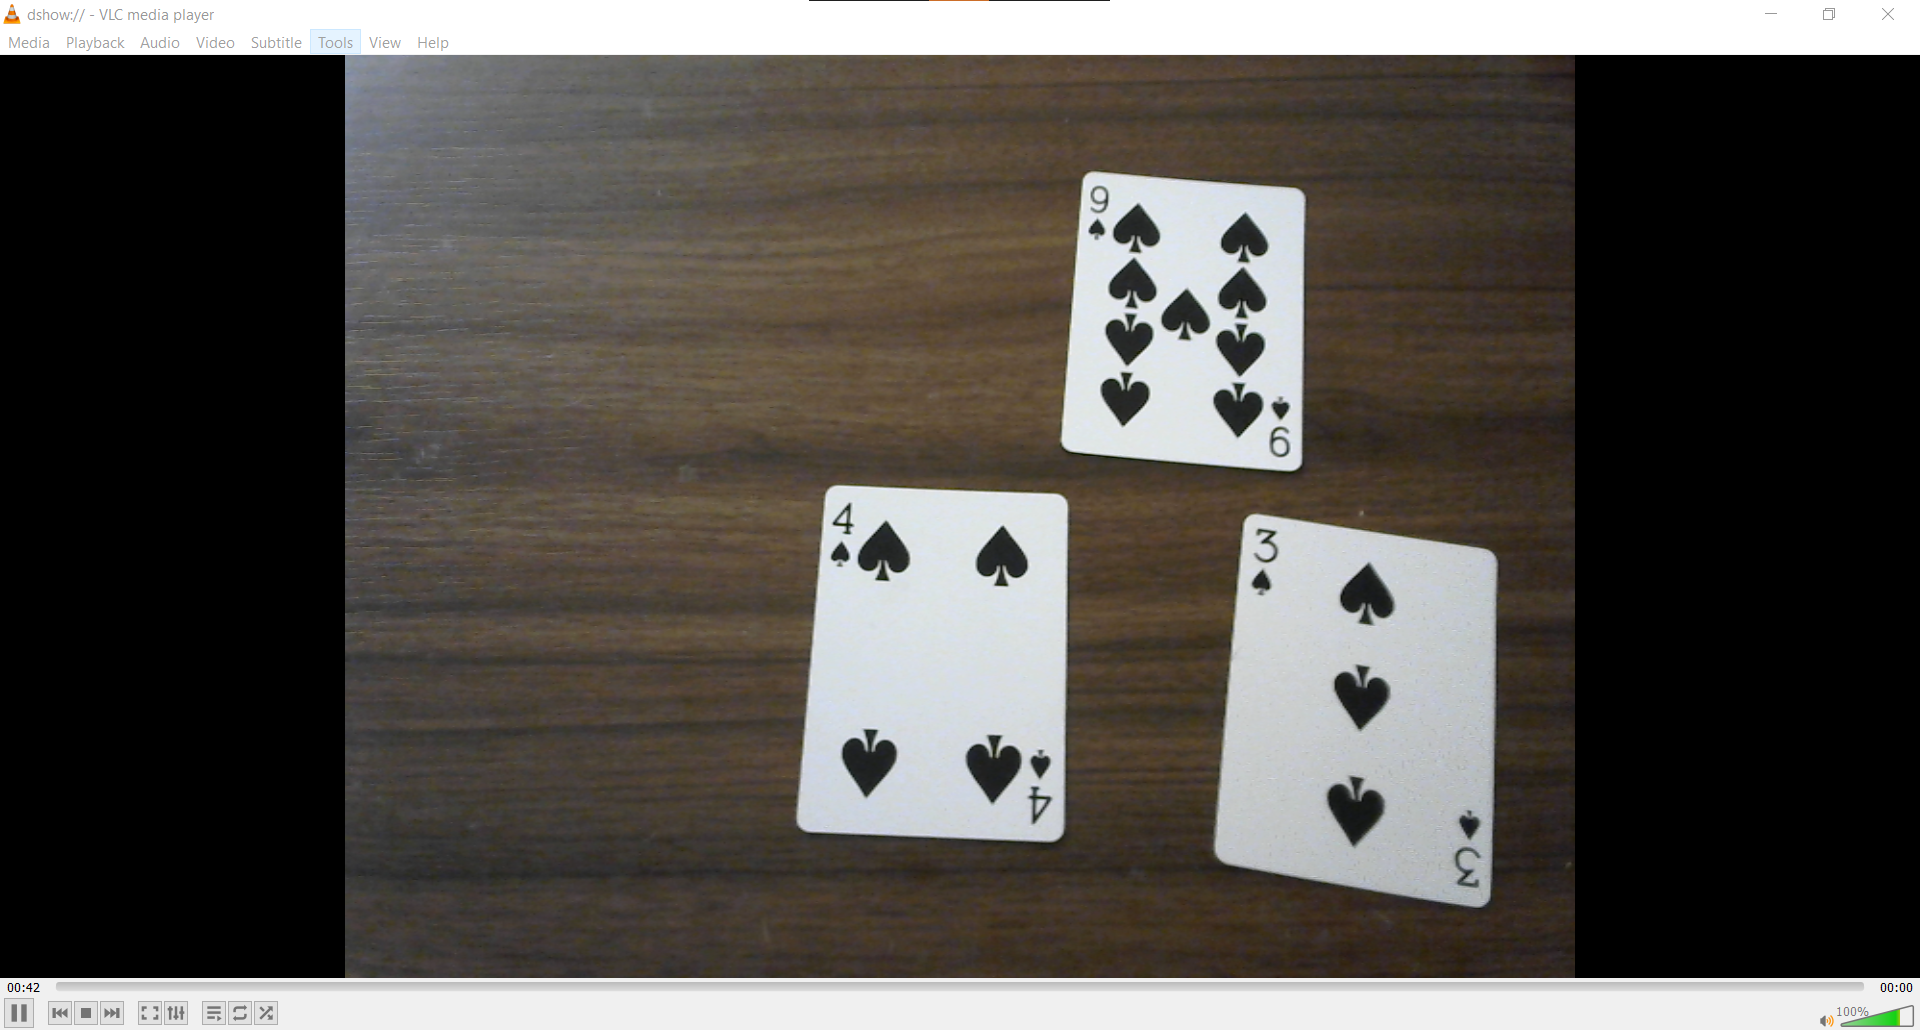
\includegraphics[scale=0.2]{vlc.png}

\section*{Algorithms}

\subsection*{Overview of recognization process}

\begin{itemize}
    \item Get mask \& contours
        \subitem Blur
        \subitem Canny edge detection
        \subitem Find contours
        \subitem Generate mask
        \subitem Get contours from the mask
    \item Get SIFT features and descriptors of each RGB channel from test image
    \item Train FLANN matcher
        \subitem Get SIFT features and descriptors of each RGB channel from template image
        \subitem Add features and descriptors to FLANN matcher
        \subitem Repeat for every template images
    \item Match \& generate recognition matrix
        \subitem Get good matches from matchers
        \subitem Calculate recognition matrix by the frequency of good matches
        \subitem Wipe out lesser frequencies with in the matrix
    \item Output final results
\end{itemize}

Most of the detailed algorithms are leveraged with OpenCV library's implementation. We put them together for our overall process.

\subsection*{1. Get mask \& contours}

Most of time, the illumination is not perfect and may makes some shadows that interfere the result. Since the poker cards are in a close shape, we can assume that the items not in close shape are background or something not interested, and make a mask to filter them out.\\
To get the mask, these steps are applied:
\begin{enumerate}
    \item Blur
        \subitem Blur image to filter out noises. Use OpenCV's implementation.
    \item Canny edge detection
        \subitem Apply edge detection that the edges will be used by the next step. Use OpenCV's implementation.
    \item Find contours
        \subitem Find contours from the edges. Use OpenCV's implementation.
    \item Generate mask
        \subitem A black image will be created first. Then the contours will be filled with white color to generate a mask. This is also the solution that some contours may reside within another contour. Use the filling method will give us the outermost shape, and that's what we need. Use OpenCV and Numpy array operations.
    \item Get contours from the mask
        \subitem After getting the mask, we are going to get the contours from the mask again. At this time, only the outermost shapes are remained, and the inner contours, like numbers, won't appear. That's how we can get the possible regions of cards from the mask now, and the contours will also be used in the later steps.
\end{enumerate}

\subsection*{2. Get SIFT features \& descriptors of each RGB channel from test image}

After having the mask, it's time to apply SIFT algorithm to the image. Here we also use OpenCV's function to detect STFI features and calculate descriptors.\\
The SIFT functions in OpenCV only accept monochrome image, so we convert color image to grayscale at first. This method is runnable to the function, however, spade and heart cards are not distinguishable since the information of color is reduced, and the shape of spade and heart is similar.\\
To solve this issue, we separate the RGB channels of the image, and regard them as 3 independent monochrome images instead of convert to grayscale. With this change, spade and heart cards can finally be recognized correctly.

\subsection*{3. Train FLANN matchers}

To match the test image with templates, a bunch of matches between the features are calculated by the FLANN matchers of OpenCV. In this step, 3 FLANN matchers are created for each RGB channel. Then, the SIFT features \& descriptors of templates are calculated just as the same way of the test image. Finally, the SIFT descriptors of templates are added to FLANN matchers respectively. The matchers will be trained automatically right before finding matches.

\subsection*{4. Match \& generate recognition matrix}

Finally, we're going to do recognition with the preparations above. The matches are calculated by the FLANN matchers with the discriptor of test image as input.\\
Now we have the possible regions of cards and the matches. How do we map the card with these regions?\\
The idea is that if a region is a specific card, the matches of the card will located within such region.\\
With this idea, we can create a matrix that take region indices as row, and template indices as column.\\
The value is the amount of matches of each template that the region contains.\\
For example:\\
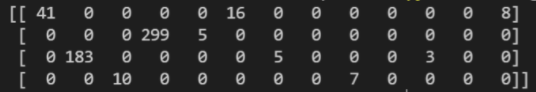
\includegraphics{matrix.png}\\
The "299" in [3, 1] means there are 299 matches of template 3 within region 1.\\
To calculate this matrix, we iterate through every matches and use OpenCV's "pointPolygonTest" function to check whether the match point is within each region. Besides, the value of the 3 channels will sum up together.\\
After that, since there will be only one specific card in a standard poker card set. We assume that one template only resides in one region, so we only leave the maximum value of the column, and zero out others. Moreover, we also zero out the column that total numbers are less then the threshold.

\subsection*{5. Output final results}

The last step is to output and visualize the final results. We iterate through every template, draw the matches of the template, and highlight the region with the maximum value that not less then the threshold. There will be a set of images with the same amount of templates.

\section*{Results}

\subsection*{Test image with 4 cards}
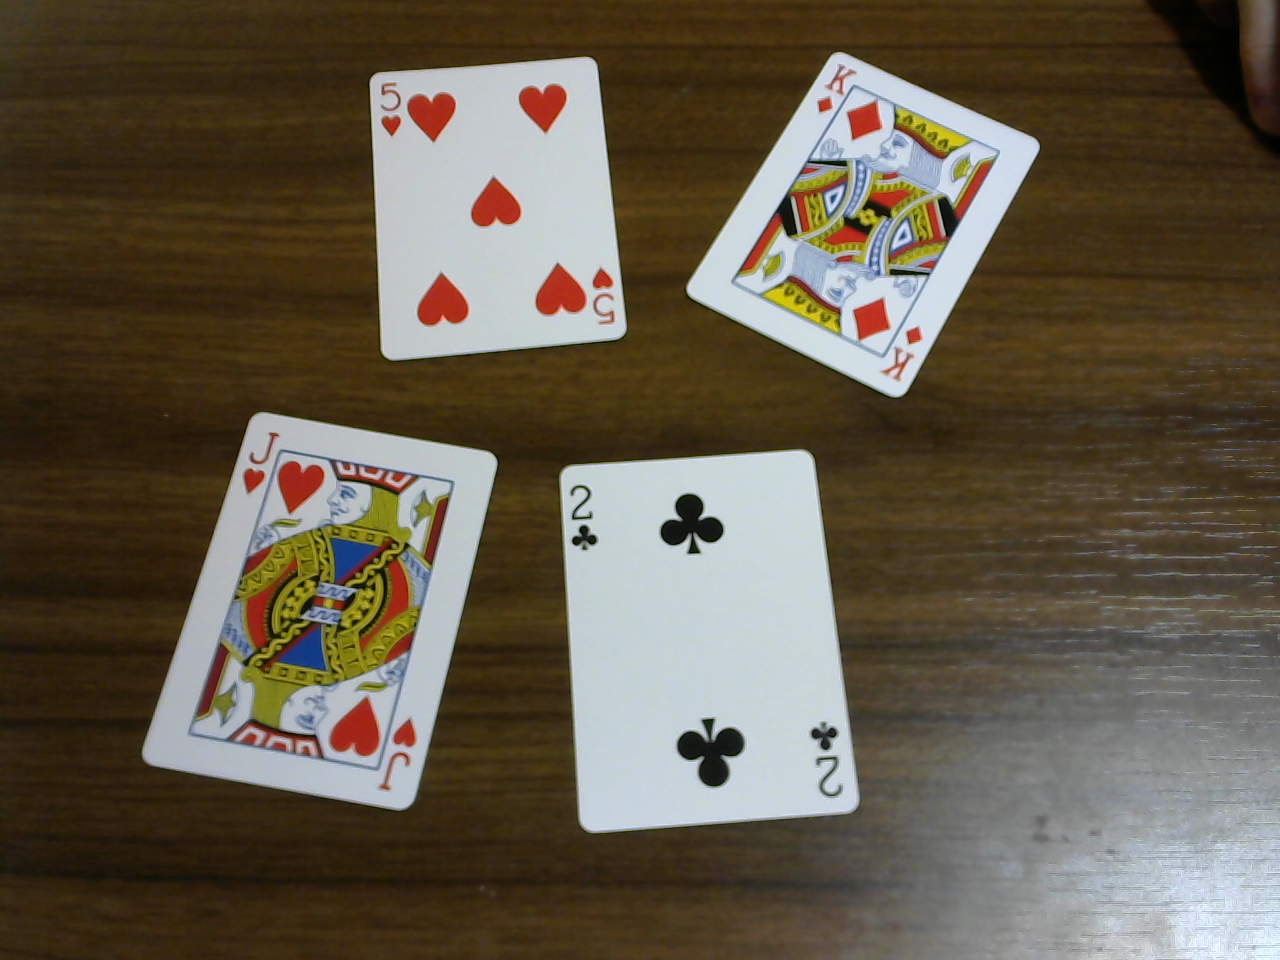
\includegraphics[scale=0.3]{testImg.png}

\subsection*{Canny edge detection}
\includegraphics[scale=0.3]{edges.jpg}

\subsection*{Contours detected from test image}
The borders of contours are drown with light green.\\
\includegraphics[scale=0.3]{contour.jpg}


\subsection*{Generated mask}
\includegraphics[scale=0.3]{mask.jpg}

\subsection*{Final result}

The left side is the test image, noted with dark red, green and blue circles indicate the SIFT features of RGB channels.\\
The right side is the images of Red, Green and Blue channels for a template, noted with SIFT features.\\
Matches of the RGB channels are drown with lines of light red, green and blue colors.\\
If a card is recognized in the test image, the region is highlighted with yellow border.

\includegraphics[scale=0.27]{match_0.jpg}\\
\includegraphics[scale=0.135]{match_1.jpg}
\includegraphics[scale=0.135]{match_2.jpg}\\
\includegraphics[scale=0.135]{match_3.jpg}
\includegraphics[scale=0.15]{match_4.jpg}\\
\includegraphics[scale=0.15]{match_5.jpg}
\includegraphics[scale=0.15]{match_6.jpg}\\
\includegraphics[scale=0.15]{match_7.jpg}
\includegraphics[scale=0.15]{match_8.jpg}\\
\includegraphics[scale=0.15]{match_9.jpg}
\includegraphics[scale=0.15]{match_10.jpg}\\
\includegraphics[scale=0.15]{match_11.jpg}
\includegraphics[scale=0.15]{match_12.jpg}

\subsection*{Additional result}

Here are 3 other test images that contains no cards.\\
\\
This is an empty scene, the recognition matrix is also an empty set\\
\includegraphics[scale=0.2]{scene1.jpg}\\
\\
These scenes contains random items. There are some closed regions within the image, however, the recognition matrix is all zero values\\
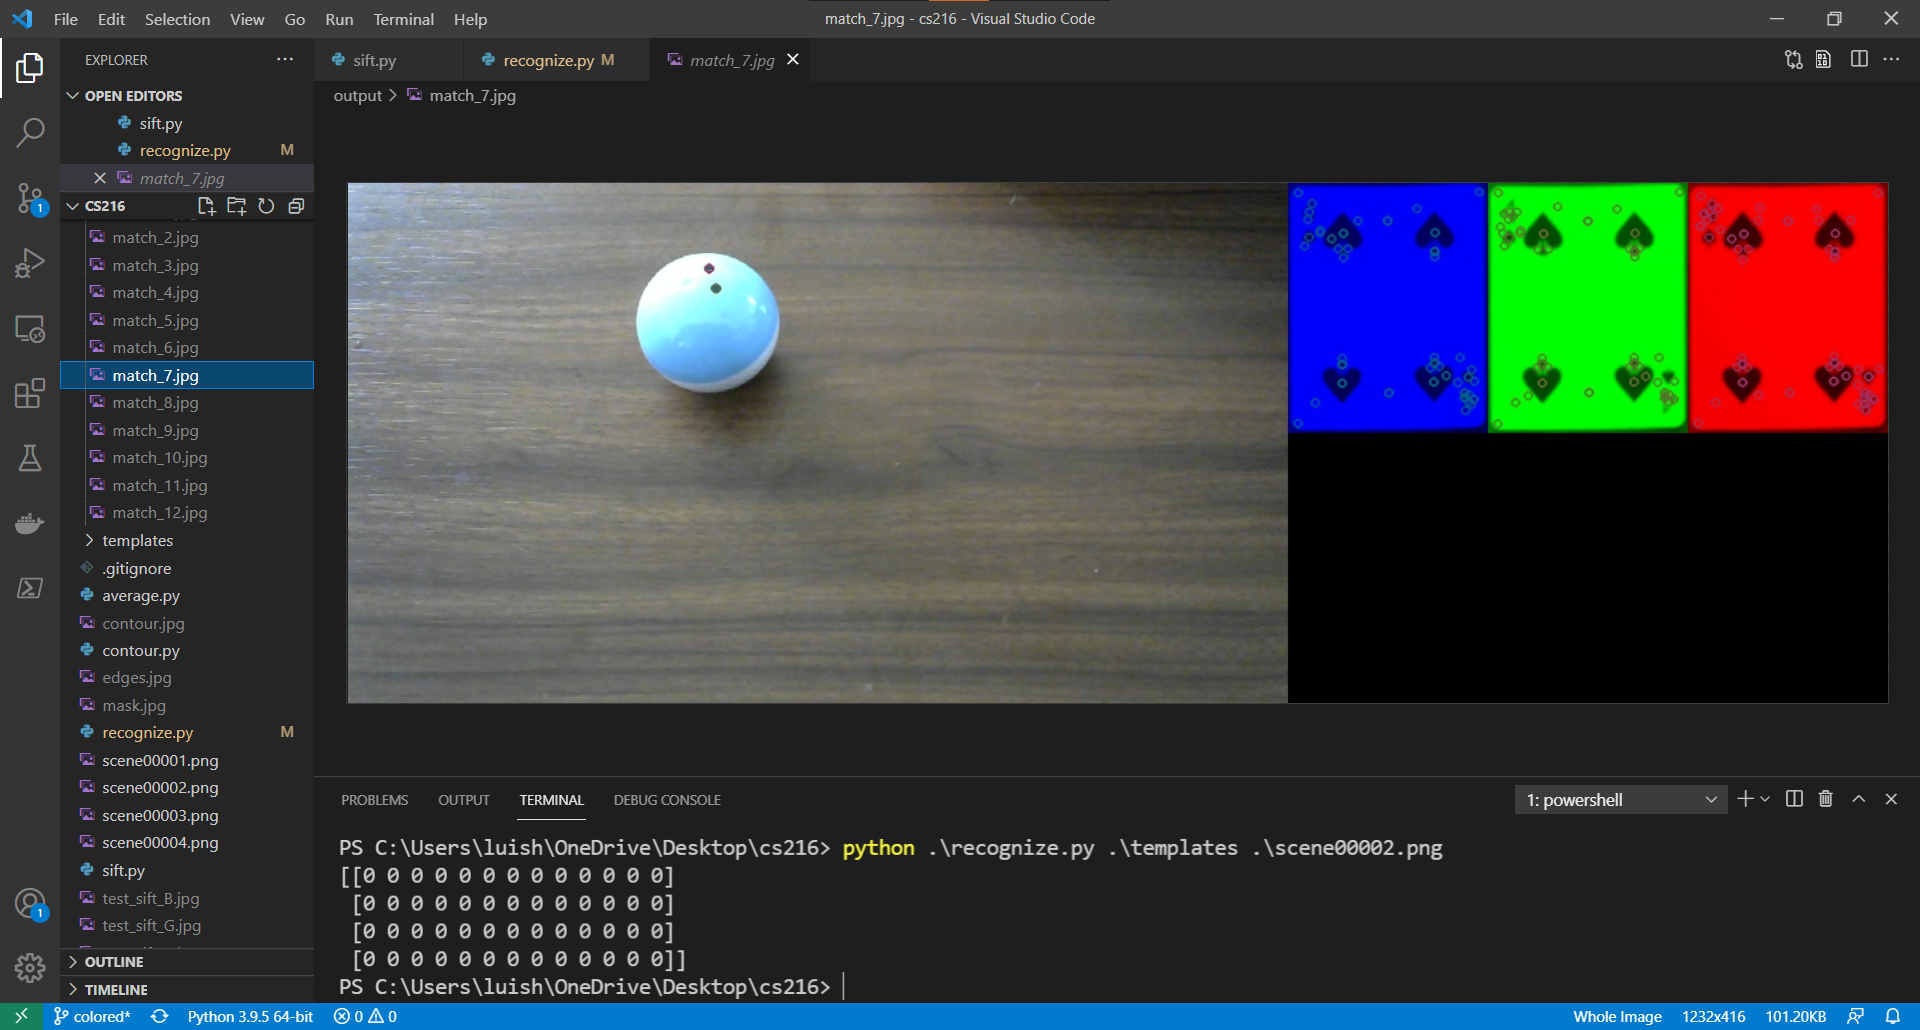
\includegraphics[scale=0.4]{scene2.png}\\
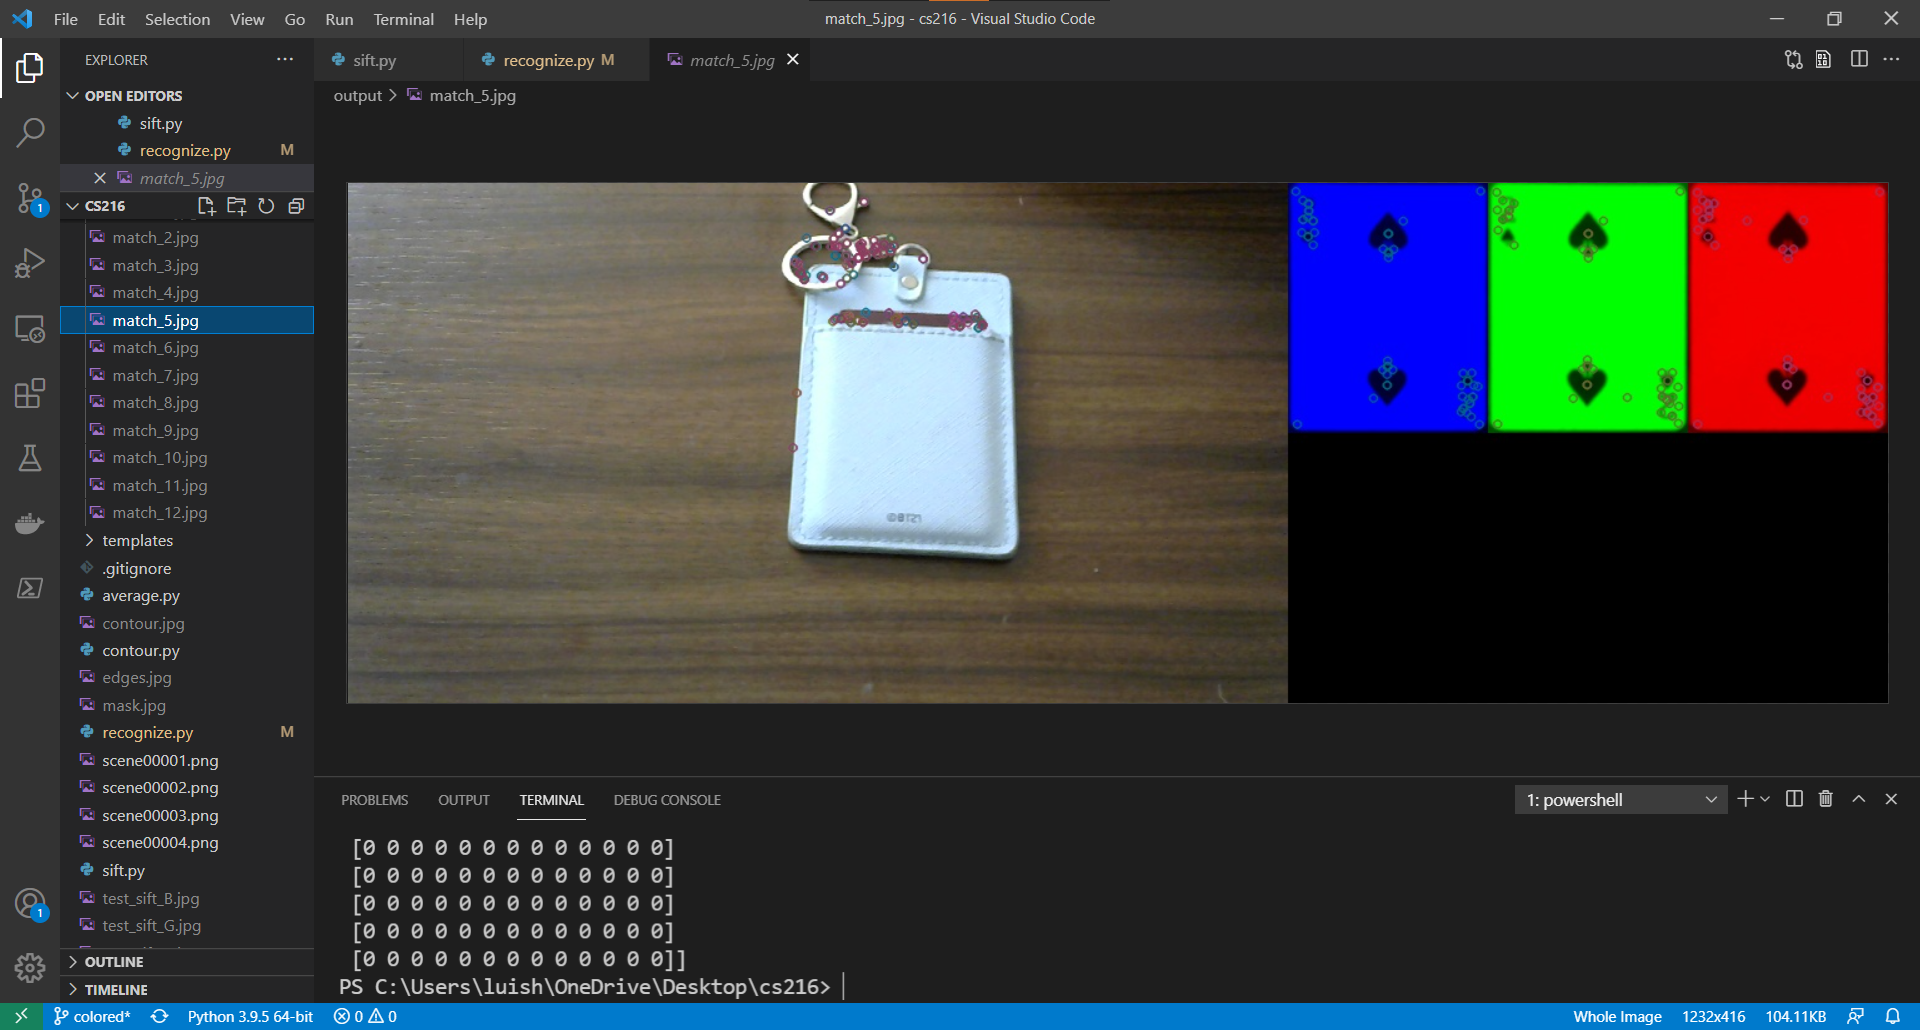
\includegraphics[scale=0.4]{scene3.png}

\section*{Assessment \& Evaluation}

\subsection*{Spotlights}

The application of OpenCV tutorial can only one template within a process. Though the output results seem like the templates are recognized separately, they are actually matched at the same time. Moreover, this project can also detect multiple templates, not only one template as the tutorial did.\\
There are some other projects we've surveyed on the GitHub that also recognize poker cards. One of them using neural network to perform recognition, however, neural network is more complex then the computer vision way, and it also cost lots of computation power. Besides, another project implements in computer vision way, but it only take numbers and shapes as template instead of the whole cards, and that may the usage only limit to poker cards. In our approach, we can easily replace poker cards with some other template images, and they may also work. This is more flexible in usage than the other projects. To summerize, this project not only able to recognize poker cards but also achieve this goal in a simpler and more scalable method.

\subsection*{Limits \& Assumptions}

There are still some limitaion and assumptions with this project.\\
\begin{enumerate}
    \item A specific card is assumed to appear only once.
    \item The whole card should be shown in the image without cut off.
    \item The cards can't overlap with each other.
\end{enumerate}
These limitations exist since we use the whole contours without more detailed analysis, and the recognition matrix only use the maximum value instead of dedicated statistical analysis. They may be solved if we have more time to improve the algorithm in such points.

\subsection*{Future works}

There are some future works we can do to improve this application.
\begin{enumerate}
    \item Extract the training process that can be explicitly trained before testing. The trained parameters can be stored somewhere and then loaded during the testing process.
    \item Find solutions for the limitations
    \item Change the input source to real-time webcam capture instead of static image.
\end{enumerate}

\section*{Resources}

\begin{itemize}
    \item OpenCV Python Tutorials\: Feature Matching
        \subitem \url{https://docs.opencv.org/master/dc/dc3/tutorial_py_matcher.html}
    \item OpenCV Python Tutorials\: Feature Matching + Homography to find Objects
        \subitem \url{https://docs.opencv.org/master/d1/de0/tutorial_py_feature_homography.html}
    \item OpenCV Python Tutorials\: Contours in OpenCV
        \subitem \url{https://docs.opencv.org/master/d3/d05/tutorial_py_table_of_contents_contours.html}
    \item \textit{Majumder, A., \& Gopi, M. (2018). Introduction to Visual Computing: Core Concepts in Computer Vision, Graphics, and Image Processing. Natick: CRC Press.}
\end{itemize}

\section*{Appendix}

These are main works in this cooperated project.
\begin{enumerate}
    \item Create mask and detect contours (Line 13-22)
        \subitem The idea of create mask from contours was coming up by myself, and the implementation is composing with functions provided by OpenCV library.
    \item Generate recognition matrix (Line 70-93)
        \subitem This idea is inspired with the Evaluation Metrics in the Assignment 1. Nevertheless, the algorithm and implementation was built on my own except for OpenCV's "pointPolygonTest" function.
\end{enumerate}

\end{document}